\begin{frame}[fragile]{CUDA}
    \begin{columns}[T]
        \begin{column}{0.48\textwidth}
            
            \vspace{0.1cm}
            \begin{center}
                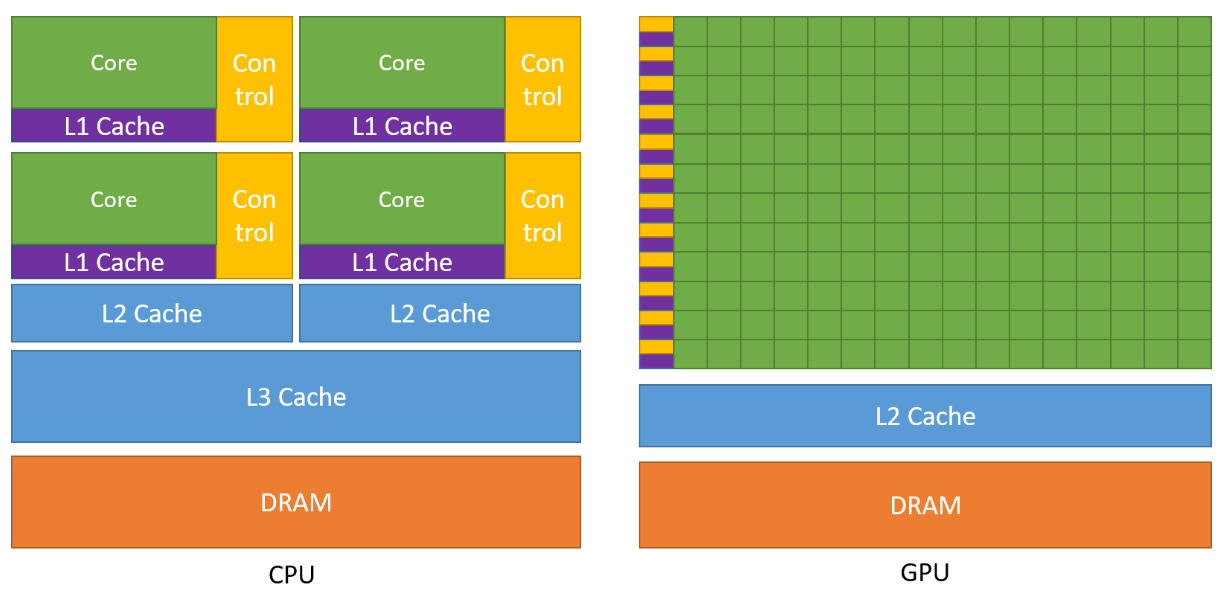
\includegraphics[width=0.7\textwidth]{Images/gpu_architecture.png}
                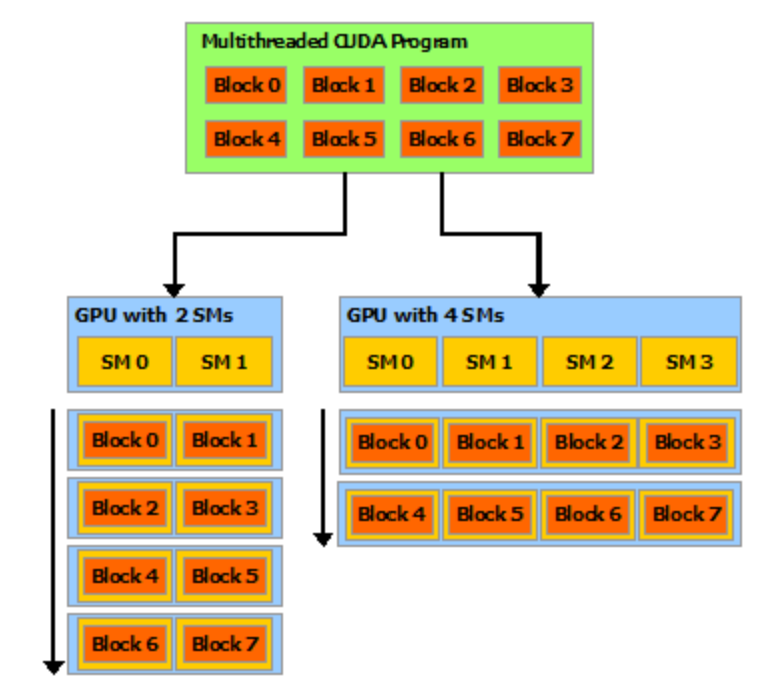
\includegraphics[width=0.7\textwidth]{Images/streaming_multiprocessor.png}
            \end{center}
        \end{column}
        
        \hfill
        \vrule
        \hfill
        
        \begin{column}{0.48\textwidth}
            \fontsize{6.5pt}{7.5pt}\selectfont
            \begin{semiverbatim}
int total_threads = blockDim.x * gridDim.x;
int id = threadIdx.x + blockDim.x * blockIdx.x;

for (int workIndex = id; 
     workIndex < a.rows * a.cols; 
     workIndex += total_threads) \{
  // Row-Major flattened execution
  int i = workIndex / a.cols;
  int j = workIndex % a.cols;
  /* ... Dot product using transposed B ... */
\}
            \end{semiverbatim}
            
            \vspace{0.2cm}
            \begin{semiverbatim}
// Threads process localized sub-matrix blocks
for (int chunk_idx = id; 
     chunk_idx < chunk_count; 
     chunk_idx += total_threads) \{
  MatrixChunk chunk = chunk_from_index(...);
  /* ... Localized loop over chunk boundaries ... */
\}
            \end{semiverbatim}
        \end{column}
    \end{columns}
\end{frame}



\begin{frame}{CUDA Performance Comparison}
    \centering Execution times are in seconds, averaged over 3 consecutive runs using 256 threads per block.
    
    \vspace{0.3cm}
    \centering
    \small
    \begin{tabular}{lrrrr}
        \toprule
        & \multicolumn{4}{c}{\textbf{Matrix Dimension ($N \times N$)}} \\
        \cmidrule(lr){2-5}
        \textbf{Algorithm Variant} & \textbf{2048} & \textbf{4096} & \textbf{8192} & \textbf{16384}  \\
        \midrule
        Transposed         & 0.19 s        & 1.50 s        & 12.91 s       & 100.55 s      \\
        Chunks             & 0.17 s        & 1.50 s        & 11.83 s       & 99.80 s       \\
        Chunks2            & 0.02 s        & 0.15 s        & 1.15 s        & 9.47 s        \\
        \bottomrule
    \end{tabular}

    \begin{center}
        \usebeamercolor[fg]{infrastructure}
        \fontsize{6.5pt}{7.5pt}\selectfont
        \texttt{Hardware | WSL2 \quad  CPU: AMD Ryzen 7 8845HS (8C/16T) \quad GPU: NVIDIA RTX 4050 (20 SM)}
    \end{center}
    
\end{frame}


\begin{frame}[fragile]{CUDA}
    \begin{columns}[T]
        \begin{column}{0.45\textwidth}
            Fast alternative
            \begin{itemize}
                \item Tile the matrices
                \item Fixed block size
                \item Copy to memory shared across threads
                \item No strong and weak scaling
            \end{itemize}
        \end{column}
        \begin{column}{0.55\textwidth}
            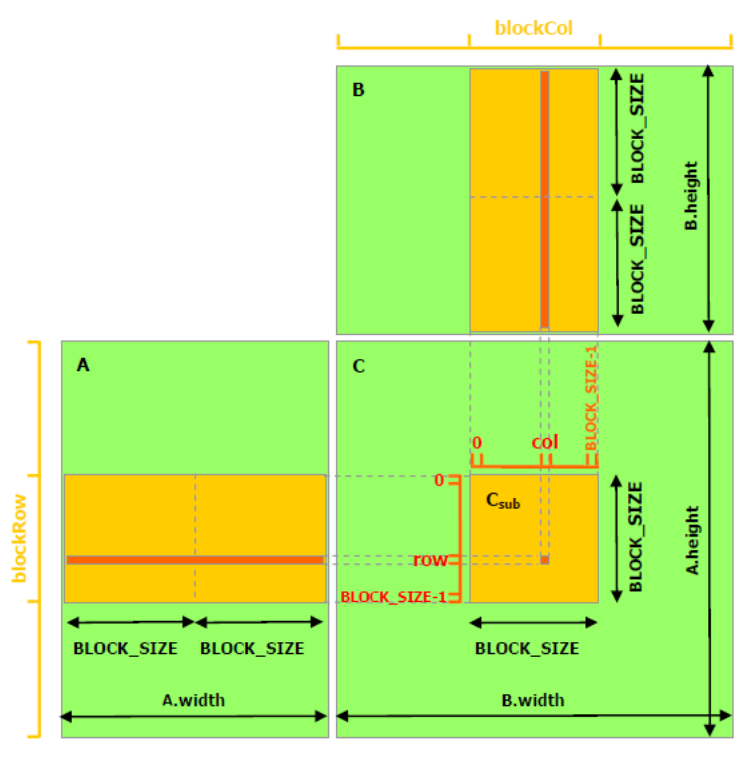
\includegraphics[width=\textwidth]{Images/cuda_blazingly_fast.png}
        \end{column}
    \end{columns}
    
\end{frame}